\documentclass[12pt]{article}

\usepackage{amsmath}    % mathematische Symbole
\usepackage{amssymb}    % noch mehr mathematische Symbole
\usepackage{german}
\usepackage[utf8]{inputenc}

\usepackage{tikz}                         % Zeichnen
\usetikzlibrary[positioning]
\usetikzlibrary{patterns}


% Für natürliche Zahlen N, reelle Zahlen R und so weiter ...
\AtBeginDocument{%
  \let\mathbb\relax
  \DeclareMathAlphabet\PazoBB{U}{fplmbb}{m}{n}
  \newcommand{\mathbb}{\PazoBB}
}
\newcommand {\N}{\PazoBB{N}}   % natürliche Zahlen
\newcommand {\R}{\PazoBB{R}}   % reelle Zahlen
\newcommand {\Z}{\PazoBB{Z}}   % ganze Zahlen
\newcommand {\Pm}{\mathcal{P}} % Potenzmenge
\newcommand {\Rm}{\mathcal{R}} % kalligravarphisches R

\begin{document}
Aufg. 4.1\\
x:
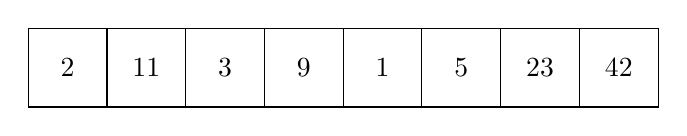
\begin{tikzpicture}[x=1cm, y=-1cm, node distance=0 cm,outer sep = 0pt]

\tikzstyle{place}=[draw, rectangle,  minimum height=1cm, minimum width=1cm, anchor=south west]

\node[place] (pos1) at (1,8) {2}; \node[place] (pos2) at (2,8) {11};\node[place] (pos3) at (3,8) {3};\node[place] (pos4) at (4,8) {9};\node[place] (pos5) at (5,8) {1};
\node[place] (pos6) at (6,8) {5}; \node[place] (pos7) at (7,8) {23};\node[place] (pos7) at (8,8) {42};
\end{tikzpicture}\\
h:
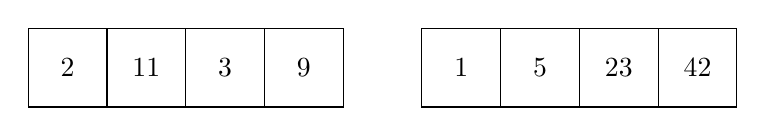
\begin{tikzpicture}[x=1cm, y=-1cm, node distance=0 cm,outer sep = 0pt]

\tikzstyle{place}=[draw, rectangle,  minimum height=1cm, minimum width=1cm, anchor=south west]

\node[place] (pos1) at (1,10) {2}; \node[place] (pos2) at (2,10) {11};\node[place] (pos3) at (3,10) {3};\node[place] (pos4) at (4,10) {9};\node[place] (pos5) at (6,10) {1};
\node[place] (pos6) at (7,10) {5}; \node[place] (pos7) at (8,10) {23};\node[place] (pos7) at (9,10) {42};

\end{tikzpicture}\\
----------------------------------------------------------------------- rekursiver Aufruf\\
x:
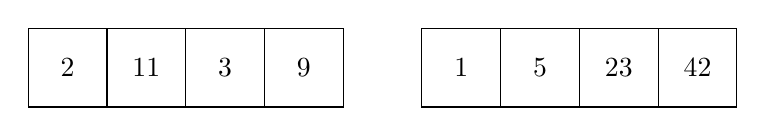
\begin{tikzpicture}[x=1cm, y=-1cm, node distance=0 cm,outer sep = 0pt]

\tikzstyle{place}=[draw, rectangle,  minimum height=1cm, minimum width=1cm, anchor=south west]

\node[place] (pos1) at (1,10) {2}; \node[place] (pos2) at (2,10) {11};\node[place] (pos3) at (3,10) {3};\node[place] (pos4) at (4,10) {9};\node[place] (pos5) at (6,10) {1};
\node[place] (pos6) at (7,10) {5}; \node[place] (pos7) at (8,10) {23};\node[place] (pos7) at (9,10) {42};

\end{tikzpicture}\\
h:
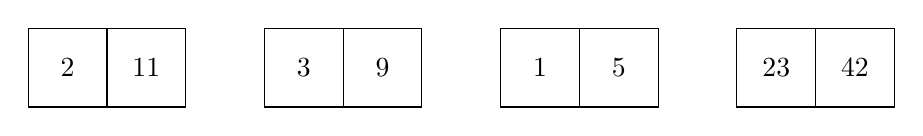
\begin{tikzpicture}[x=1cm, y=-1cm, node distance=0 cm,outer sep = 0pt]

\tikzstyle{place}=[draw, rectangle,  minimum height=1cm, minimum width=1cm, anchor=south west]

\node[place] (pos1) at (1,10) {2}; \node[place] (pos2) at (2,10) {11};\node[place] (pos3) at (4,10) {3};\node[place] (pos4) at (5,10) {9};\node[place] (pos5) at (7,10) {1};
\node[place] (pos6) at (8,10) {5}; \node[place] (pos7) at (10,10) {23};\node[place] (pos7) at (11,10) {42};

\end{tikzpicture}\\
----------------------------------------------------------------------- rekursiver Aufruf\\
x:
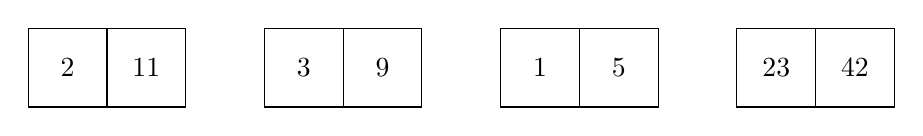
\begin{tikzpicture}[x=1cm, y=-1cm, node distance=0 cm,outer sep = 0pt]

\tikzstyle{place}=[draw, rectangle,  minimum height=1cm, minimum width=1cm, anchor=south west]

\node[place] (pos1) at (1,10) {2}; \node[place] (pos2) at (2,10) {11};\node[place] (pos3) at (4,10) {3};\node[place] (pos4) at (5,10) {9};\node[place] (pos5) at (7,10) {1};
\node[place] (pos6) at (8,10) {5}; \node[place] (pos7) at (10,10) {23};\node[place] (pos7) at (11,10) {42};

\end{tikzpicture}\\
h:
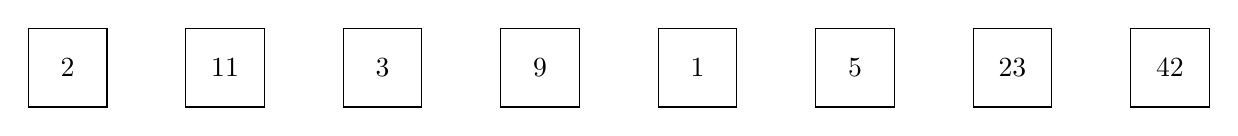
\begin{tikzpicture}[x=1cm, y=-1cm, node distance=0 cm,outer sep = 0pt]

\tikzstyle{place}=[draw, rectangle,  minimum height=1cm, minimum width=1cm, anchor=south west]
\node[place] (pos1) at (1,10) {2}; \node[place] (pos2) at (3,10) {11};\node[place] (pos3) at (5,10) {3};\node[place] (pos4) at (7,10) {9};\node[place] (pos5) at (9,10) {1};
\node[place] (pos6) at (11,10) {5}; \node[place] (pos7) at (13,10) {23};\node[place] (pos7) at (15,10) {42};

\end{tikzpicture}\\
----------------------------------------------------------------------- rekursiver Aufruf\\
x:
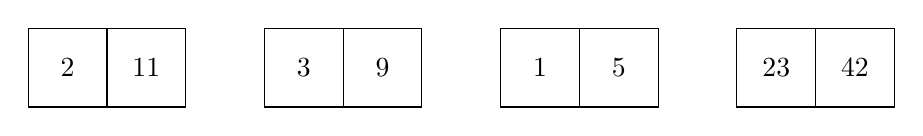
\begin{tikzpicture}[x=1cm, y=-1cm, node distance=0 cm,outer sep = 0pt]

\tikzstyle{place}=[draw, rectangle,  minimum height=1cm, minimum width=1cm, anchor=south west]

\node[place] (pos1) at (1,10) {2}; \node[place] (pos2) at (2,10) {11};\node[place] (pos3) at (4,10) {3};\node[place] (pos4) at (5,10) {9};\node[place] (pos5) at (7,10) {1};
\node[place] (pos6) at (8,10) {5}; \node[place] (pos7) at (10,10) {23};\node[place] (pos7) at (11,10) {42};

\end{tikzpicture}\\
----------------------------------------------------------------------- \\
x:
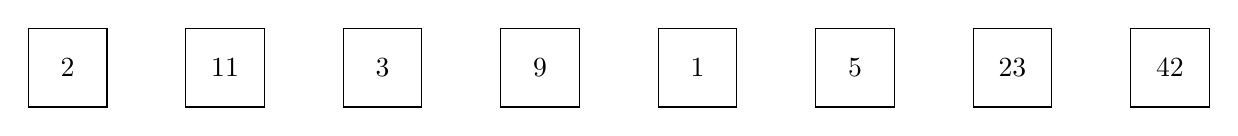
\begin{tikzpicture}[x=1cm, y=-1cm, node distance=0 cm,outer sep = 0pt]

\tikzstyle{place}=[draw, rectangle,  minimum height=1cm, minimum width=1cm, anchor=south west]

\node[place] (pos1) at (1,10) {2}; \node[place] (pos2) at (3,10) {11};\node[place] (pos3) at (5,10) {3};\node[place] (pos4) at (7,10) {9};\node[place] (pos5) at (9,10) {1};
\node[place] (pos6) at (11,10) {5}; \node[place] (pos7) at (13,10) {23};\node[place] (pos7) at (15,10) {42};

\end{tikzpicture} \\
h:
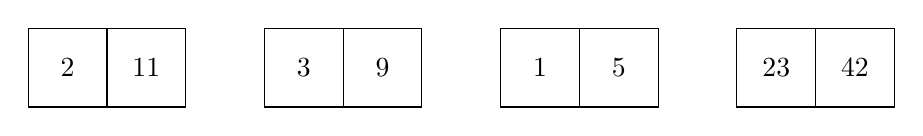
\begin{tikzpicture}[x=1cm, y=-1cm, node distance=0 cm,outer sep = 0pt]

\tikzstyle{place}=[draw, rectangle,  minimum height=1cm, minimum width=1cm, anchor=south west]

\node[place] (pos1) at (1,10) {2}; \node[place] (pos2) at (2,10) {11};\node[place] (pos3) at (4,10) {3};\node[place] (pos4) at (5,10) {9};\node[place] (pos5) at (7,10) {1};
\node[place] (pos6) at (8,10) {5}; \node[place] (pos7) at (10,10) {23};\node[place] (pos7) at (11,10) {42};

\end{tikzpicture}\\
----------------------------------------------------------------------- \\
h:
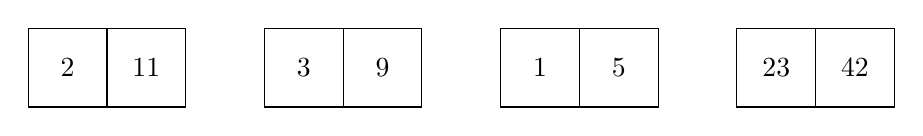
\begin{tikzpicture}[x=1cm, y=-1cm, node distance=0 cm,outer sep = 0pt]

\tikzstyle{place}=[draw, rectangle,  minimum height=1cm, minimum width=1cm, anchor=south west]

\node[place] (pos1) at (1,10) {2}; \node[place] (pos2) at (2,10) {11};\node[place] (pos3) at (4,10) {3};\node[place] (pos4) at (5,10) {9};\node[place] (pos5) at (7,10) {1};
\node[place] (pos6) at (8,10) {5}; \node[place] (pos7) at (10,10) {23};\node[place] (pos7) at (11,10) {42};

\end{tikzpicture}\\
x:
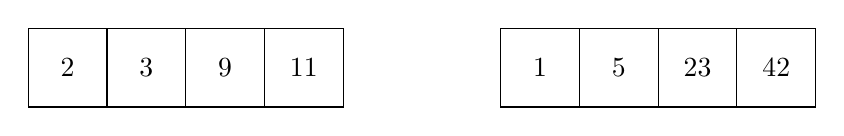
\begin{tikzpicture}[x=1cm, y=-1cm, node distance=0 cm,outer sep = 0pt]

\tikzstyle{place}=[draw, rectangle,  minimum height=1cm, minimum width=1cm, anchor=south west]

\node[place] (pos1) at (1,10) {2}; \node[place] (pos2) at (2,10) {3};\node[place] (pos3) at (3,10) {9};\node[place] (pos4) at (4,10) {11};
\node[place] (pos5) at (7,10) {1}; \node[place] (pos6) at (8,10) {5}; \node[place] (pos7) at (9,10) {23};\node[place] (pos7) at (10,10) {42};

\end{tikzpicture}\\
----------------------------------------------------------------------- \\
h:
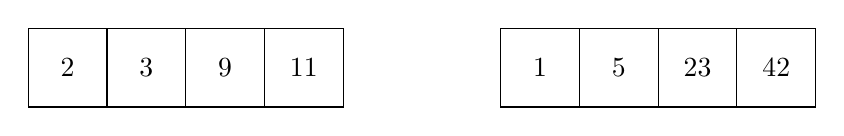
\begin{tikzpicture}[x=1cm, y=-1cm, node distance=0 cm,outer sep = 0pt]

\tikzstyle{place}=[draw, rectangle,  minimum height=1cm, minimum width=1cm, anchor=south west]

\node[place] (pos1) at (1,10) {2}; \node[place] (pos2) at (2,10) {3};\node[place] (pos3) at (3,10) {9};\node[place] (pos4) at (4,10) {11};
\node[place] (pos5) at (7,10) {1}; \node[place] (pos6) at (8,10) {5}; \node[place] (pos7) at (9,10) {23};\node[place] (pos7) at (10,10) {42};

\end{tikzpicture}\\
x:
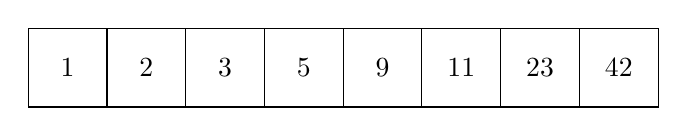
\begin{tikzpicture}[x=1cm, y=-1cm, node distance=0 cm,outer sep = 0pt]

\tikzstyle{place}=[draw, rectangle,  minimum height=1cm, minimum width=1cm, anchor=south west]

\node[place] (pos1) at (1,10) {1}; \node[place] (pos2) at (2,10) {2};\node[place] (pos3) at (3,10) {3};\node[place] (pos4) at (4,10) {5};
\node[place] (pos5) at (5,10) {9}; \node[place] (pos6) at (6,10) {11}; \node[place] (pos7) at (7,10) {23};\node[place] (pos7) at (8,10) {42};

\end{tikzpicture}\\





\end{document}
